\chapter{Introduction}


\section{Overview}
\label{overview}

The design of a cockpit is a complex and lengthy process.
The engineering team must constantly manage a variety of complex design constraints, requirements, human factors, mission context, and technical limitations.
To manage the complexity of the project, the design is reviewed throughout the process to ensure requirements are being met.
 One important part of these reviews is an evaluation from the future users of the cockpit -- i.e.\ the pilots or astronauts.
Feedback from pilots can validate the current design, highlight potential issues, or even discover major design flaws.
The tools used for the pilot evaluations evolve as the design matures, becoming more and more realistic to the eventual flight mission.
Initially, evaluations may be done from paper studies of the design, progressing to engineering mockups, then flight simulators, and finally flight tests.
These are the typical tools used throughout the design of a cockpit, though the specifics of each can depend on the project and resources available.
For example, a flight simulator can range in fidelity from a desktop simulator to a motion-base simulator.
Just as with the simulator, the mockup can range in fidelity from as simple as a foamboard structure with printouts of cockpit instruments to a machined, full scale construction of the size and layout of the craft in design.
The distinguishing feature between a mockup and a simulator is that a mockup is non-functional.
The mockup is typically built early in the design process, before a full simulator can be developed.
Often, the main purpose of a mockup is for ergonomic studies and it is not as effective of a tool for pilot evaluations as a simulator.

The simulator can provide a mission context to the evaluation pilots, and with a functioning simulation they can determine the workload of their flight tasks and identify any potential issues.
However, this comes at a cost of significant time and money to develop the flight simulator.
Additionally, by the time the cockpit design is ready for the development of a simulator it can be no longer feasible to undertake large design changes.
If the pilots are unsatisfied with the design at this stage, the deficiencies risk being ignored under pressure of schedule and cost.
Instead, the remaining deficiencies of the cockpit are expected to be overcome through additional crew training.
This represents a cost in training throughout the lifetime of the vehicle, typically measured in decades, and ``unknown'' deficiencies of the human-machine system are often discovered too late in accident reports.

As opposed to the simulator, mockups are more likely to be developed during the early stages of the design process where large scale changes are more frequent and exact sizing and placement of components may not be complete.
Mockups are built to provide designers a physical representation of the cockpit or flight deck in design instead of committing to building a fully functioning simulator.
The mockup as a pilot evaluation tool is limited, and the reason for this is the same reason it is adaptable to large changes: the components are non-functional.
Mockups are built without functioning instruments or displays so that changes can be made more rapidly.

In this work, we describe a tool named the ``Rapidly Reconfigurable Research Cockpit'' (R3C) created to bridge the gap between mockup and simulator.
To achieve this, we have designed and built a prototype of a virtual environment that adds the immersion and interactivity benefits of a more functional simulator to a non-functional geometric mockup.
 Evaluation pilots, while seated in the mockup, wear an immersive head-mounted display that provides a high fidelity and dynamic virtual view of the cockpit panel, interior, and exterior window views.
The head-mounted display is tracked and gaze-registered, enabling the cockpit visuals to be overlaid on the low fidelity physical mockup.
The motion and gestures of the cockpit evaluator are tracked using an unobtrusive hand tracker to read the users' inputs on the non-functioning cockpit instruments.
This provides the essential interactivity to turn the mockup from a non-functioning device into a functioning simulator.
With the R3C system, an evaluator can wear a head-mounted display to provide an immersive virtual-visual layer registered with the physical world in the mockup and still retain their ability to touch and feel the cockpit.
As opposed to a full simulator it does not require a time and cost expensive hardware integration, instead it can be defined in software.
Similarly, as opposed to using a virtual reality simulator without any physical representation, combining with the mockup provides a more realistic simulation since it becomes coupled with the tactile sense.
This virtual environment combines the roles of mockup and simulator, bringing the accompanying benefits of a full simulator to the benefits of early stage design mockups: faster and more drastic redesign iterations.

Our work does not aim to supersede any existing process or design philosophy, but rather provides a tool that human systems integration engineers can use to enhance their process.
Specifically, we aim to improve the iterative design process of cockpit design by reducing cost and time for the redesign cycles by bringing a more functional tool to the early stages of design.
The importance of the iterative process has been highlighted in many design approaches.
For example, quoting from \citet{nasa_nasa_2015}:
\begin{displayquote}
Human-centered design \textelp is characterized by early and frequent user involvement, performance assessment, and an iterative design-test-redesign process.
\end{displayquote}
Another goal of the R3C system is to not only increase the number of iterations, but to improve the feedback from the evaluations.
The use of a mockup for design evaluation is standard in the industry.
\citet{zea_development_2012} reported on design of a cockpit architecture for the then in-development DreamChaser spacecraft.
Three mockup versions were constructed, and they found that ``a significant amount of knowledge acquired from the mockups was not attainable through computer models''.
A physical mockup that also acts as a functioning simulator will help to improve the feedback of the cockpit evaluations.
Quoting from \citet{sexton_cockpitcrew_1988}:
\begin{displayquote}
\textins{The test pilots} must consider the design in a mission context, as if they are using the systems while flying -- the more realistic the testing environment, the more meaningful the findings.
\end{displayquote}
By allowing the cockpit evaluators to use the mockup as a functioning simulator, the feedback will be more effective with the context of the mission being provided with the virtual layer.
The R3C system will allow for more iterative cycles with more meaningful feedback from pilots early in the design process.
This combination will lead to a more optimized cockpit design.
Eliminating the design deficiencies early will not only lead to cost savings in the design process, but the eventual design will reach a more optimized state.
This will reduce crew training and errors throughout the life of the vehicle.
The cost savings and safety benefits of a more optimized design can be enormous, both during the design stage and beyond.

The overall objective is to provide an unprecedented ability to optimize a new spacecraft cockpit layout via rapid, low-cost design iterations by integrating state-of-the-art technologies in virtual reality, hand tracking and 3D printing.
The work presented in this dissertation reports on the design and integration of the R3C prototype, experimental results both to understand how humans perform with the prototype and to evaluate the performance of the prototype as a design tool.

The prototype system of the ``Rapidly Reconfigurable Research Cockpit'' (R3C) that has been developed consists of a virtual reality (VR) headset, an optical hand tracking device, and 3D printed cockpit surfaces (Figure \ref{fig:intro_r3c}).
The VR head-mounted display (HMD) provides a virtual-visual view of the cockpit environment.
A challenging aspect of immersive VR simulations is to provide a sense of touch.
We solve this by using 3D printed instruments co-located with the virtual environment, a technique commonly called ``passive haptics''.
 The instruments remain inert and non-functioning in the real world, but appear fully functional in the virtual world presented to the user.
They can be modeled to the exact shape of a cockpit instrument being designed, and printed within a matter of hours.
Instead of requiring the mockup instruments to have functioning buttons, the input of the pilot is read using the hand tracker to provide the interaction with the cockpit.
The optical based hand tracker measures the real-time position of the pilots' hand to determine if they are touching a button.
The hand tracker also displays their hand in the virtual world for the user, as the use of an HMD blocks the view of one's own limbs.
Additionally, the use of the hand tracker allows for a more thorough examination of the hand movement of evaluation pilots in a new cockpit design than is typically possible.

\begin{figure}
    \centering
    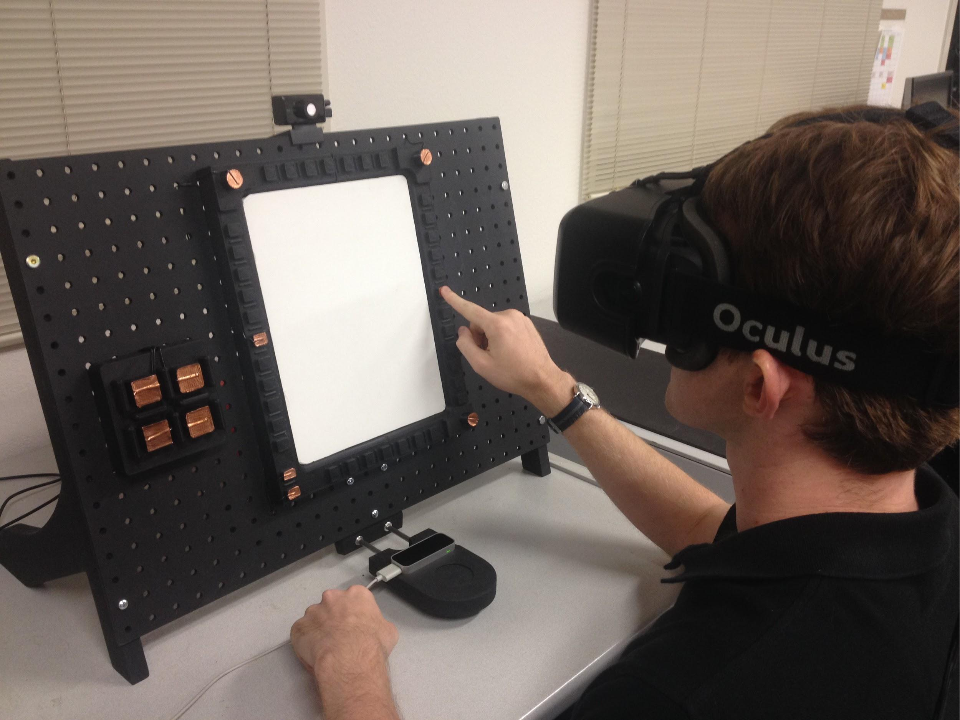
\includegraphics[width=\textwidth]{r3c_no_callout.png}
    \caption{The Rapidly Reconfigurable Research Cockpit prototype.}
    \label{fig:intro_r3c}
\end{figure}

The combination of these technologies allows an existing mockup to be used as a functioning simulator with visuals overlaid on top of screens and/or out-the-window views, and with functioning buttons on the instrument.
With merged mockup and simulator functions, adjustment of the developing cockpit can be made simpler, cheaper, and more quickly turned around.
The result of employing this virtually-enhanced mockup should be a human interface that is truly optimized, which can result in increased safety and efficiency, as well as reduced crew workload/fatigue.

The R3C prototype has been the technical base for the research performed in this work.
The three main tracks of the research can be summarized in these aims:
\begin{enumerate}
    \item Create a virtual reality system with passive haptics and hand tracking that allows for evaluation of early design cockpits (Chapter \ref{chap:prototype}).
    \item Validate the technical approach and evaluate the performance of subjects in the virtual reality environment with passive haptics (Chapters \ref{chap:pointing} and \ref{chap:ph_exp}).
    \item Evaluate the use of the prototype in a mock design evaluation study to determine differences in standard performance metrics and subject feedback from using the R3C system (Chapter \ref{chap:de_exp})
\end{enumerate}
The technical approach and development of the prototype is described in Chapter \ref{chap:prototype}.
Three experiments with human subjects have been performed and are reported on to support these aims in Chapters \ref{chap:pointing}, \ref{chap:ph_exp}, \ref{chap:de_exp}.
The first experiment (Chapter \ref{chap:pointing}) asked subjects to repeatedly target one of four buttons on the panel under different conditions, testing differences between real versus virtual world as well as passive haptics versus no passive haptics (mid-air reaching).
We recorded time to completion and accuracy to the button center.
%It was found that the virtual world caused a slight but significant degradation in time for the reaching movement, but no significant change in accuracy.
%The accuracy requirement is more important for our application of safety-critical human-machine interfaces, where accuracy requirements often prevail over movement time.
The second experiment (Chapter \ref{chap:ph_exp}) had subjects perform a Fitts' Law task in different conditions to further characterize the difference between using passive haptics and mid-air reaching.
%The recorded 3D hand trajectory data will also be used to develop the metric for Aim 3 (which is being called the ``task familiarity'' metric or model in this report).
%By using the Fitts' circle for Experiment 2, we can use the Fitts' throughput as a truth measure of familiarity to train and test the model upon.
Additionally, this experiment had a more extensive subject survey to collect the opinions of the subjects, especially on the differences between using passive haptics and mid-air reaching.
The final experiment (Chapter \ref{chap:de_exp}) performed the same design evaluation study using the R3C system and a traditional simulator.
This was done to compare the results to determine where, if any, differences were obtained from the evaluation results.
Subjects were split into two groups, one using the R3C and the other a touchscreen simulator.
Two instrument designs were presented to each subject and they were asked to perform the same task on both.
Afterwards, their comments about the two designs were collected.
Performance measures of the task were also recorded and analyzed.
The goal of the experiment was to determine where subject feedback and performance may differ between an evaluation study using R3C and one using a touchscreen.
The differences found were described and discussed.

\section{Background}

To frame this research, this section will summarize relevant previous work as well as background on the dependent measures used in the experimental work.
The first few sections summarize different tracks of virtual reality research: it's use in design and prototyping, different haptic environments, and the evaluation of virtual environments.
Next, input device evaluation research such as Fitts' Law is discussed, highlighting work that has been performed in virtual environments.
Finally, a summary of various human reaching trajectory research is given to understand how the human formulates trajectories in a virtual environment.

\subsection{Virtual Environments for Design}

Recent advancements in virtual reality technology has renewed interest in the benefits of virtual prototyping, and its use has been increasing across industries - manufacturing \citep{choi_virtual_2015}, assembly \citep{pontonnier_designing_2014}, automotive \citep{bordegoni_mixed_2012,lawson_future_2016}, and medicine \citep{nagendran_virtual_2013}.
The term virtual prototyping (VP) is an encompassing term for a variety of virtual interfaces and/or interactions.
%and any virtual environment can exist on a spectrum from full virtuality to full reality \citep{milgram_taxonomy_1994}.
The use of virtual environments in design processes is well established.
%Virtual manufacturing was described by \citet{shukla_virtual_1994} as ``the use of computer models and simulations of manufacturing processes to aid in the design and production of manufactured products.''
Many design and engineering teams adopted virtual reality early in order to enhance their prototyping process.
\citet{brooks_jr_whats_1999} reviewed the (at the time) current use of virtual reality applications in industry.
A number of engineering design firms had already seen the potential for using virtual reality set ups in design reviews, though display applications were typically wall-projections instead of a head-mounted display.
John Deere claimed \$80K of savings from preliminary mockup costs from using a VR system and Chrysler performed ergonomic reviews using a head-mounted system, though the HMDs at the time were very heavy and low resolution \citep{brooks_jr_whats_1999}.
\citet{abate_haptic-based_2009} investigated the use of haptic interactions for virtual reality training of assembly and maintenance task, and performed a usability assessment which found technicians preferred the use of haptics in a virtual maintenance task.

\citet{aromaa_suitability_2016} reviewed the use of virtual prototypes for human factors/ergonomics (HFE) evaluation.
They found that the fidelity of a VP may not affect subjective results, but that task performance can be affected, hindering the utility of the evaluation itself.
This is supported by findings that decreased presence (the feeling that the simulation is real) can negatively affect task performance \citep{youngblut_relationship_2003}.
\citet{lawson_future_2016} provided recommendations for incorporating VP in the automotive industry for HFE evaluation, including using haptic feedback and marker-less body tracking.
They found that the use of markers can encumber the participant, affecting evaluation results.

Flight simulation was one of the first applications of virtual environments, and the use of virtual environments for training and development of new cockpits has persisted throughout the years \citep{hancock_human_2008}.
Virtual reality simulators for aviation have recently become a more active track of research.
\citet{wan_mrstudio:_2011} used an augmented reality approach to register a virtual-visual layer on top of a mockup of a commercial aircraft cockpit for design and evaluation but did not describe any interaction methods.
\citet{yavrucuk_low_2011} combined an immersive head-mounted display with hand tracking gloves to provide a virtual simulator of a helicopter.
They did not use any haptic feedback and users interacted with the instruments using the hand tracking, with no physical mockup.
\citet{aslandere_virtual_2015} had a similar technical setup with a head-mounted display and tracked gloves.
Their report focused on the virtual button interaction using a hand tracker.
They found that the collision volume for a virtual button interaction did not impact the interaction, but a more realistic hand avatar increased efficiency.
The first appearance of work similar to ours was by \citet{schiefele_simple_1998} in Germany, which also used a head-mounted display (HMD) to replace the visuals of a flight simulator (though technology has drastically changed in HMDs since their work).
They recreated only the positions of the panels with a flat plate and then used a magnetic hand tracker for reading the pilot input.
A short usability study was presented, and they found that users could activate switches, knobs and dials in less time with the physical panel than without (i.e.\ reaching into mid-air).


\subsection{Virtual Tactile Environments}
\label{virtual-tactile-environments}

One of the challenges of virtual environments has been presenting the user with a tactile sensory input that matches the visual sensory inputs they are experiencing.
Many haptic glove products have been created that attempt to simulate this with motor vibrations.
Since they are attached to your body, they cannot provide any external stopping force, so the simulation can break down when interacting with rigid objects.
Another technique is using a stylus mounted to a 6-DOF actuator that can simulate external forces.
These have been used for many studies with the application of surgical tasks, when a tool would be used in the real scenario as well.
The focus of this work is the idea of \emph{passive haptics}, whereby the tactile environment is recreated to provide the sense of touch, including external forces.
The disadvantage is that the tactile environment cannot dynamically change during the simulation.
Some researchers have attempted to create dynamic passive haptics \citep{mcneely_robotic_1993, tachi_construction_1994}, which use a robotic arm to deliver the appropriate tactile experience to the user as they reach into the virtual world.
This approach quickly becomes complicated and expensive.
Others have tried approaches to morph the virtual world to adapt to a generic passive haptic device \citep{kohli_exploiting_2009,kohli_redirected_2012}, which can work only for small discrepancies.
Fortunately, the adaptability during a simulation of the passive haptic environment is not a requirement for the use case of a pilot evaluating a new cockpit interface.
We still retain the ability to quickly change the environment in between simulation sessions via 3D printing new parts.

Previous work with passive haptics, though limited, have shown it to provide benefits.
\citet{insko_passive_2001} investigated the impact of passive haptics on generic virtual environments.
It was found that the passive haptics increased the sense of presence felt by users.
An experiment had two groups complete a maze in a virtual environment, one group with passive haptics on boundaries, and one without.
After training, the passive haptic group bumped into far fewer obstacles than the group without.

\citet{borst_evaluation_2005} created a ``mixed'' haptic virtual environment, whereby they combined an active haptic glove with a passive haptic panel.
The panel provided the stopping force and depth location of the interface, while the glove haptics provided the finer details of the buttons, switches and dials.
They compared subjects performing tasks on the panel using the glove by itself (no panel), the passive haptics by itself (no glove), as well as their mixed condition (panel and glove).
They found the glove by itself consistently performed worse than the other two, but overall no significant difference existed between passive haptics and their mixed haptic condition.

An important reason for the use of haptic feedback is that co-located haptic feedback has been shown to increase performance of tasks in a virtual environment \citep{swapp_interaction_2006}.
\citet{bouguila_effect_2000} found that haptic feedback improved the perception of depth in a stereoscopic virtual environment.
The ability to perceive depth would be an important factor for the use of a virtual environment for human factors evaluation.

\subsection{Virtual Environment Evaluation}
\label{virtual-environment-evaluation}

It is notoriously hard to quantify the effectiveness of a virtual environment (VE).
One can report on quantitative measures of the virtual reality (VR) setup such as latency, field of view, resolution and others, but in the end the only important measure is whether the user finds the virtual environment convincing.
This can also change depending on the user -- one user could find a VE convincing while another finds it intolerable.
The effectiveness of a VE is often linked to the sense of \emph{presence}, defined by \citet{witmer_measuring_1998} as ``the subjective experience of being in one place or environment, even when one is physically situated in another.''
\citet{sheridan_musings_1992} argued that presence is a subjective sensation that necessitates a subjective measure.
Two of the more popular post-questionnaires that have been developed are the Presence Questionnaire (PQ) \citep{witmer_measuring_1998} and the Slater-Usoh-Steed (SUS) questionnaire \citep{slater_depth_1994}.
The former (PQ) consists of 32 questions that cover various factors of presence such as sensory, control, distraction and realism.
The SUS questionnaire consists of only 6 questions and is focused on the feeling of presence.
\citet{nystad_comparison_2004} found the PQ to be more sensitive to technology and interaction methods, while the SUS fits better to the definition of presence.
This suggests PQ may be better suited for our work when comparing between conditions, but SUS could be useful as a general evaluation of the overall system.
The increased presence with passive haptics found by \citet{insko_passive_2001} previously mentioned is an important finding we aim to replicate for our virtual environment.

Presence is an important measure as it has been shown to correlate with performance in the virtual environment \citep{youngblut_relationship_2003}.
A high sense of presence increases the feeling that the objects shown in the virtual environment are real and the interactions are the same as they would be in the real world.
It also provides the user with a better memory of the environment \citep{dinh_evaluating_1999}.

We also hypothesize that our system will reduce the amount of arm fatigue experienced by the operator compared to a mid-air pointing virtual environment (i.e.\ no tactile workstation present).
This common phenomenon in virtual environments is often called ``gorilla arms'', as people feel that their arms are too heavy to support after prolonged use reaching out into the void.
A measure of this arm fatigue is not included in the standard presence questionnaire.
The literature does not contain a large volume of experiments that measure arm fatigue.
Qualitative measures include a Likert scale, the ISO-9241-9 ``Assessment of Comfort and Fatigue'' and the Borg scales (RPE and CR10).
The Borg CR10 performs favorably to the other scales for measures of exertion \citep{grant_comparison_1999}.
Recently, a quantitative approach has been proposed that uses optical tracking of the arm and wrist which validated well against a Borg CR10 scale \citep{hincapie-ramos_consumed_2014}.
Adapting their software to our system would be out of scope (and requires more upper-limb measurement than we are currently capable of) but the validation against the Borg CR10 scale is promising.

\subsection{Input Device Evaluation}
\label{input-device-evaluation}

For decades one of the most important empirical models in the Human-Computer Interface (HCI) community has been Fitts' Law.
The basis of the model is a method to predict the movement time of a user towards a target.
The average movement time can be accurately predicted using just the size and distance to the target after empirically determining the model parameters.
It has been used to evaluate new input devices to determine how fast a user can move to a target (e.g.\ mice, trackballs, joysticks), as well as a guideline for interface designs (ensuring that target areas are the right size).
A summary of the field is presented here, with notable contributions and similar work following.
Fitts' Law used in the context of virtual environments and our work is then discussed.

\subsubsection{Fitts' Law}
\label{fitts-law}

\citet{fitts_information_1954} originally reported on his experiments of targeted reaching movements between varying target sizes, and compared the correlated he discovered to information theory models.
He postulated that the entire control system of the human, from motor control to visual and proprioceptive feedback, can process information at a certain maximum rate, and the bandwidth of the channel must be derivable from the physical parameters of the target.
Fitts' adapted Shannons' Theorem from information theory for the bandwidth of a channel in the presence of a signal and noise \citep{shannon_communication_1949}.
The distance to the target (\emph{D}) is considered the signal, and the width of the target (\emph{W}) is considered to be the noise (Figure \ref{fig:intro_fitts}).
This analogy allowed Fitts' to create a formula for the \emph{index of difficulty} (\(\text{ID}\)) of a target:

\begin{equation}
    \mathrm{ID} = \log\left(\frac{2D}{W}\right)
    \label{eq:intro_id}
\end{equation}

It was found experimentally that the index of difficulty is linearly correlated to \emph{movement time} (MT), the time taken to move between the start and the target.
This leads to the equation that is now known as Fitts' Law:

\begin{equation}
    \mathrm{MT} = a + b \cdot \mathrm{ID}
\end{equation}
where \emph{a} and \emph{b} are the parameters of the linear regression, which are determined experimentally.
A typical experiment consists of subjects performing movements to a range of targets with varying indices of difficulty, and recording their movement time.
The data is then fit to a linear regression to find \emph{a} and \emph{b}.

\begin{figure}
    \centering
    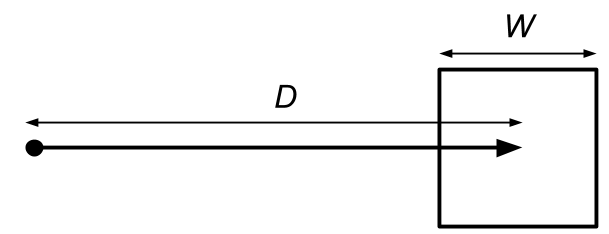
\includegraphics[width=0.5\textwidth]{fitts_dimensions.png}
    \caption{The dimensions of a Fitts' Task (\emph{D} = distance, \emph{W} = width)}
    \label{fig:intro_fitts}
\end{figure}

Since its original formulation, refinements to the model have focused on the formula for index of difficulty, \(\text{ID}\), and the definition of its dependencies, width and distance.
\citet{crossman_speed_1957} suggested a very important refinement called the adjustment for accuracy.
This provides a correction to the \(\text{ID}\) to compensate for the task which is actually performed by the subject as opposed to the task that was asked to be performed.
For example, if a subject is presented with two large targets close together ($D << W$), then they tend to aim towards the inner edges of the targets instead of the center, effectively using a much smaller target width.
The adjustment for accuracy replaces the width, \(W\), with the \emph{effective width}, \(W_{e}\).
The basis for this adjustment is that the information theory basis for Fitts' Law expects that the ``noise'' of the target width induces a 4\% error rate \citep{mackenzie_fitts_1992}.
If more or less than 96\% of the target hits are successfully within the target, then the target width is adjusted with the adjustment for accuracy to fit the target error rate of 4\%.
Motor tasks have been shown to be a Gaussian distribution \citep{crossman_feedback_1983,woodworth_accuracy_1899}, thus 96\% of target endpoints will be within 4.133 standard deviations (\(\sigma\)).
The effective width is thus calculated with the standard deviation from the endpoint data:
\begin{equation}
W_{e} = 4.133\sigma
\end{equation}
It is recommended to calculate the effective width for each subject in each condition as it is sensitive to both between and within subject variability \citep{soukoreff_towards_2004}.
The effective width can then be used to calculate an \emph{effective index of difficulty}, \(\text{ID}_{e}\).
The effective width described here is for one dimensional targets, but there are extensions to 2D targets as well \citep{murata_extending_2001}.

The form of the logarithmic term in the index of difficulty equation (Eq.\ \ref{eq:intro_id}) has encountered some debate over the years.
Fitts did not describe the reasoning for including the factor of two in his original formulation, and \citet{welford_fundamentals_1968} suggested a modification that provided a better fit for low values of index of difficulty.
The Welford modification simply adds
\begin{equation}
    \mathrm{ID} = \left( \frac{D}{W} + 0.5 \right).
\end{equation}
A more recent variation proposed by \citet{mackenzie_note_1989} suggests that by comparing to Shannons' Theorem, as Fitts originally proposed as the theoretical basis for his work, then the form should be,
\begin{equation}
    \mathrm{ID} = \left( \frac{D + W}{W} \right) = \left( \frac{D}{W} + 1 \right)
\end{equation}
which has been widely adopted in literature as the Shannon's Formulation.
As well as being based in the original theoretical underpinnings of Fitts' Law, the mathematical structure of this formulation will not produce a negative index of difficulty with real, positive dimensions, unlike the original equation.

The first use of Fitts' Law in the human-computer interface (HCI) community was with \citet{card_evaluation_1978}, comparing the use of a mouse, joystick and keys for text selection.
This led to an extensive use of Fitts' Law in the HCI field, both as a way to evaluate input devices and a design law for user interfaces.
Best practices of using Fitts' Law have been developed, and the standard ISO-9241-9:2000 provided guidelines for the use of Fitts' Law in evaluation of input devices \citep{international_organization_for_standardization_iso_2000}.
Most notably, it was suggested to use the ISO-9241 ``Fitts' circle'' for evaluations of 2D tasks (Figure \ref{fig:intro_fitts_circle}).
This input pattern has been widely adopted in literature, and provides a standard for comparing across studies.

\begin{figure}
    \centering
    
\includegraphics[width=0.5\textwidth]{fitts_circle.png}
    \caption{ISO-9241 Fitts' Circle or multi-directional tapping task.}
    \label{fig:intro_fitts_circle}
\end{figure}

\citet{soukoreff_towards_2004} present a review of the best practices for designing and performing a Fitts' law experiment, including the use of the Shannon Formulation and the ISO-9241 ``Fitts' circle''.
They also advise the use a large range of ID values, ideally from 2 to 8 bits.

When Fitts' Law is used to evaluate input devices, the metric of comparison is often \emph{throughput}.
Throughput (TP) is defined as the index of difficulty (ID) over the movement time (MT).
\begin{equation}
    \mathrm{TP} = \frac{\text{ID}}{\text{MT}}
\end{equation}
The units of throughput are bits per second, and it represents the information capacity of the input device.
A higher throughput indicates that the human is able to convey more information (\emph{bits}) through one input device versus another in a given time (\emph{per second}).
\citet{soukoreff_towards_2004} recommend the use of throughput as the measure for comparing experimental conditions as well.
One of the advantages of using throughput is that it combines speed and accuracy requirements through the use of the index of difficulty.
Throughput has been validated to be invariant to subjects prioritizing speed or accuracy \citep{mackenzie_fitts_2008}.

The debate on which form and refinement of Fitts' Law is the best to use continues to this day \citep{drewes_only_2010,hoffmann_which_2013}, and this work will not attempt to settle this debate.
%\tinytodo{rewrite this}However, the understanding of the origin of Fitts' Law, best practices and the many forms of the equations will greatly influence the design and success of the experiments performed.
Since no form of the equations have been rejected outright in the literature, it is recommended to perform analysis with all versions and note if any significant differences in major conclusions result \citep{soukoreff_towards_2004}.

\subsubsection{Dimensionality of Fitts' Law}\label{dimensionality-of-fitts-law}

Throughout the Fitts' Law literature, one of the main differences between experiments is how many dimensions the subjects can move their targeting device (hand, stylus, cursor).
There are two dimensionalities to consider when discussing Fitts' Law experiments: the dimensionality of the task, and the dimensionality of the movement.
The dimensionality of the task refers to the number of dimensions the targets are placed in.
A 1D task means the targets are aligned along a single axis, whereas a 2D task has them located on a plane (such as the Fitts' circle in Figure \ref{fig:intro_fitts_circle}).
The dimensionality of the movement refers to how many dimensions the subjects need to move when moving between the targets.
For example, the original Fitts' Law task was a 1D task as the targets were varied in width along the movement direction, but sufficiently long in the perpendicular dimension, removing that dimension as a variable.
The movement, however, was effectively 2D, as the subjects could (and needed to) lift up from the table to move between targets.

The popularity of Fitts' Law in the HCI field has led many researchers to focus on the use of Fitts' Law on a 2D computer screen controlled by a mouse.
This is a 2D task, with a constrained 2D movement.
For our application, the movement we are interested in is a 2D task with 3D movement since the buttons on a cockpit panel are configured in approximately a single plane, with pilots reaching towards them in unconstrained 3D movement.
There are some newer studies that present this task and movement dimensionality, as it is analogous to the use of a touchscreen device.
Some have proposed minor variations to the formulation of Fitts' law to adjust for touchscreens \citep{bi_ffitts_2013,sears_high_1991}, but others have found the original formulation to perform well \citep{mackenzie_fitts_2015}.
There are also studies discussed in the next section that perform this task in a virtual environment.

Refinements have been proposed to account for the possible effects of extending the task dimensionality to 2D, such as the bivariate target model \citep{accot_refining_2003, mackenzie_extending_1992, wobbrock_error_2008}.
Some work has also explored this for 3D tasks, introducing a trivariate model \citep{grossman_pointing_2004} and corrections for 3D placement of targets \citep{cha_extended_2013, murata_extending_2001}.
These experiments place targets in a truly 3D space, with of course 3D motion required of the user.
The use of a Fitts' circle on the 2D plane effectively removes the need for these accommodations, as the targets are symmetric and have the same width when approached from any direction.

\subsubsection{Fitts' Law in Virtual Environments}\label{applying-fitts-to-virtual-environment}

Fitts' Law has been used in evaluating virtual environments and their input devices.
\citet{chun_evaluating_2004} evaluated a set of 3D stereo displays with a single haptic-enabled stylus using a Fitts' tapping task.
They did not have well-fit regressions, but this could have been due to a small range of ID values used (2-3), targets being placed in 3D space (a 3D task with 3D movement), with random order (making the sequence of the task un\-learn\-able), and averaging across subjects before completing the regression.
\citet{teather_evaluating_2010} performed a similar task and also found a poor fit of the regression in the fully 3D task.
One condition performed a mid-air 2D planar task with 3D movement, and no significant difference in throughput was found compared to the same task with constrained 2D motion.
\citet{liu_comparing_2009} performed a planar multi-directional Fitts' task with a stereoscopic display, and compared virtual world to real world results, finding movement time twice as long in the virtual condition.
The trajectories were analyzed to determine where the extra movement time was spent, which is discussed in the next section (\nameref{human-targeting-motion}).
\citet{teather_pointing_2011} performed an ISO-9241 Fitts' circle task in a CAVE virtual environment (stereoscopic projection on walls) with a motion tracked stylus, comparing performance with and without a passive haptic on the plane of the targets.
They found increased throughput with the passive haptics, but throughput performance was lower than they had expected.

One of the few experiments that utilize Fitts' Law in an immersive HMD was performed by \citet{kohli_redirected_2012} who focused on evaluating ``discrepant'' (warped virtual space) virtual environments to fool the user of the nature of the physical world.
They had the subjects perform an ISO-9241 Fitts' circle on a panel placed in front of them, and in some conditions the panel was rotated in the virtual world but not in the real world or vice-versa to create the discrepancy.
The subjects' hand movement was warped to compensate for this.
Their non-discrepant condition (when virtual and real were at the same angle) should compare to our results with passive haptics.

\citet{coelho_pointing_2014} evaluated the LeapMotion hand tracker (the same technology used in our work) in a 3D Fitts' task (with visual feedback on a computer screen), but did not perform a Fitts' model analysis, comparing only time.
\citet{seixas_one_2015} performed an ISO 9241-9 Fitts' circle task with the LeapMotion.
Their goal was to compare a gesture based selection technique, and they provide a Fitts' throughput comparison between that and direct mid-air selection.
Ours is the first work to perform a Fitts' Law evaluation with a passive haptic, immersive VR, and the LeapMotion.

\subsection{Human Targeting Motion}
\label{human-targeting-motion}

In one of the earliest experiments to measure trajectories of human targeting motions, \citet{woodworth_accuracy_1899} discovered that there are two distinct phases of the targeting motion: a ballistic phase and a corrective phase.
Subjects typically perform the bulk of their movement in the ballistic phase, often considered more of an open-loop or feed-forward mechanism, and as they near the target switch to a feedback, closed-loop, corrective phase \citep{elliott_control_1999}.

Experiments in virtual environments have shown that users typically spend more time in the corrective movement phase than when performing the same task in a non-virtual environment \citep{liu_comparing_2009}.
However, this work was completed for a mid-air interaction, so it is an open question whether the introduction of passive haptics would reduce the corrective phase `penalty' for targeting motions in a virtual environment.
%We can quantitatively investigate this question with the use of our virtual environment.
\citet{mackenzie_three-dimensional_1987} showed that there was correlation between the target size and the time of the deceleration phase for a Fitts' task, suggesting that subjects will adapt their trajectory for accuracy requirements.
Our application to a cockpit environment is one where accuracy demands are often more important than time demands for manipulation of instruments.

Other metrics have been developed in the literature to evaluate the trajectory of a targeting motion.
\citet{meyer_optimality_1988} developed a parsing criterion to divide the trajectory into submovements and defined three types: return from overshoot, accelerate due to undershoot, and slowing towards target.
\citet{mackenzie_accuracy_2001} presented a set of accuracy measures for targeting motions based on trajectory information.
They were developed to compliment a Fitts' input device evaluation.
The measures are named target re-entry, task axis crossing, movement direction change, orthogonal direction change, movement variability, movement error, and movement offset.
They quantify types of movement that are not along the ideal straight-line path from start to goal.

\subsection{Summary}
\label{summary}

The combination of immersive virtual reality simulator with an inert passive haptic has not been extensively tested in the virtual reality literature.
Other approaches at immersive haptics have focused on creating a dynamic environment, but our application of a static cockpit does not need to change geometrically during the simulation (not to be confused with our re-configurability between simulations).
Unobtrusive hand tracking (requiring no gloves on the user) like the one we are using has been highlighted as important for human factors evaluations.
The integration of these new hand tracking technologies is a further innovation, allowing us to provide interactivity with the passive haptics.

To evaluate this new virtual environment, we use two validated measures -- presence and Fitts' Law.
Fitts' Law is a well validated and actively used model for evaluating both input devices and interfaces.
To date there have been only a few uses of Fitts' Law in immersive head-mounted display virtual environments.
As of our knowledge, no one has performed a Fitts' Law experiment in a virtual environment using the new generation optical hand trackers (i.e.\ the LeapMotion we are using).
A Fitts' Law characterization is an important step to take to evaluate the system we have created, and provides a standard means of comparison across previous and future literature.
Additionally, the trajectories of the targeting motions can be used to further analyze the motion.
Past research has found that the use of a virtual environment affects the trajectory but no work has investigated the effect of passive haptics.

Virtual environments have found much use in design and prototyping.
Some research has started to investigate the use of various forms of augmented and virtual reality for these tasks.
Our combination of technology has not been tested in the context of a design evaluation tool.

\section{Research Questions}
\label{hypotheses}

The research presented in this work consists of three experiments with human subjects to answer our fundamental research questions.
As is natural with research work, our research questions and motivations evolved with the findings of the previous experiment.
Presented here are a summary of the major research questions that were investigated with the experimental work.
The questions are further detailed in their respective experiment chapters.

\begin{itemize}
    \item Can the technical approach of a mockup providing passive haptics with a virtual-visual overlay using a head-mounted display be used successfully?
    \item Can a user select a button in the R3C prototype with the passive haptics and hand tracker as quickly and accurately as one in the real world?
    \item Does the use of passive haptics change the performance of subjects targeting a button in the virtual environment?
    \item Does the use of passive haptics increase the presence of subjects using the virtual environment?
    \item Does the use of passive haptics change the trajectory formation of subjects targeting a button in the virtual environment?
    \item Can the R3C prototype be used effectively as a design evaluation tool?
    \item How does the R3C prototype compare to other design evaluation tools?
\end{itemize}

\section{Summary}

We have introduced our goals and motivation for the creation of the Rapidly Reconfigurable Research Cockpit prototype, a system for providing a higher fidelity evaluation of new cockpit designs while still retaining a low iteration cost.
The background for the experimental work has been described and the open research questions that we explore in this work have been summarized.
In the following chapters, we first describe the technical work to create the Rapidly Reconfigurable Research Cockpit (Chapter \ref{chap:prototype}), before reporting on the three experiments and their results (Chapters \ref{chap:pointing}-\ref{chap:de_exp}).
